\section{Оптический отклик полупроводниковой метаповерхности на основе германия.}

\subsection{Постановка задачи. Параметры образца.}
В полупроводниковых наноструктурах с субволновым периодом решетки ожидаться резонанс в следствии многократного рассеяния  волны накачки \cite{mftiOpt}. В данной структуре (рис. \ref{base1}) ожидался резонанс в конце ИК диопазона.

\begin{figure}[h]
	\centering
    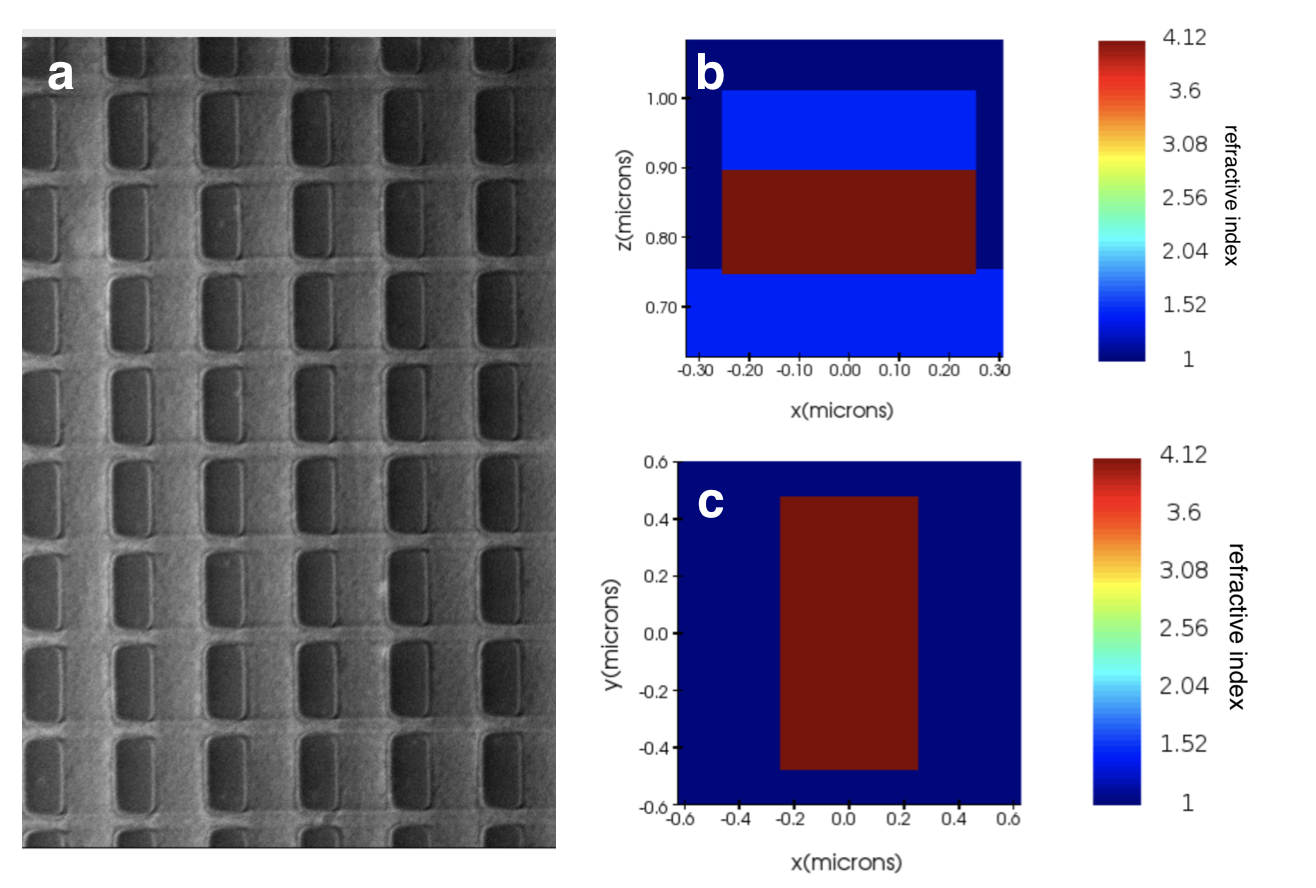
\includegraphics[width=0.8\linewidth]{images/base1.png}
	\caption{На рисунке изображен снимок метаповерхности. В качестве подложки используется $CaF_2$. На подложке  горизонтальным  0,75мкм и вертикальным шагом 0,25мкм разположенны кирпичике германия(Ge) толщиной 0,15мкм. На верху каждого кирпичека германия расположен слой стекал ($SiO_2$) толщиной $\sim 0,1$мкм. Изображение на вставке - вид модели с верху. Цветная шкала справа показывает показатель преломления различных структур, изображенных на картинке)}
	\label{base1}
\end{figure}

\subsection{Исследование линейного отклика метаповерхности на основе германия}
\hspace{2mm}
Периодическая структура освещаться плоской волной накачки. Монитора a1(рис.  \ref{base2}а) расположен выше источника электромагнитных волн и измеряет отражение структуры (рис. \ref{1:wave_eq}c), а монитор a2(рис. \ref{base2}а) расположен ниже кирпичика германия и измеряет пропускание структуры (рис. \ref{base2}b). Резонанс можно наблюдать как на спектре пропускание(рис. \ref{base2}с) так и на отражения структуры (рис \ref{base2}с).  Из графиков видно, что резонанс достигаться на длине волны  $\lambda_{RES} \approx 2$мкм. 
\hspace{2mm}
 Вероятнее всего наблюдаемый резонанс возникает из-за геометрических особенностей метаповерхности - частицы расположины с таким периодом, что в результате многократного отражения волны накачки, генерируется квазиволновая мода, которую мы и наблюдаем в резонансе.
\begin{figure}[h]
	\centering
    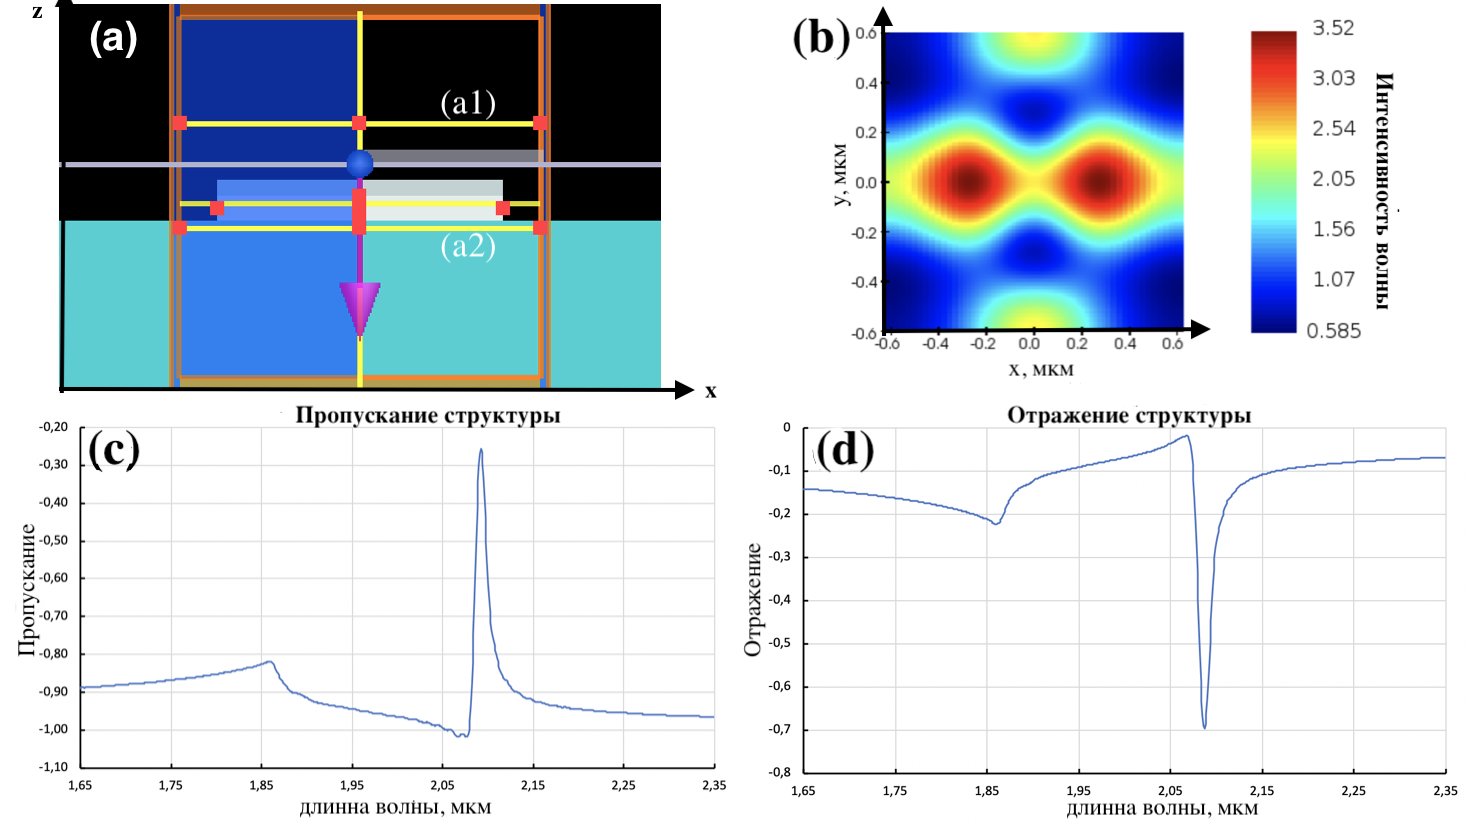
\includegraphics[width=0.9\linewidth]{images/expert.png}
	\caption{\textbf{(a)}На рисунке изображен 1 период метаповерхности. Монитор \textbf{а1}, меряющий отражение структуры, \textbf{а2} - монитор, меряющий пропускание структуры. На графиках \textbf{(b, c)} предсавленны показания этих мониторов. Резонанс достигаться при длинне волны накачки $\lambda_{RES} = 2,085$мкм. На \textbf{(d)} показано распределение электрического поля в германии во время резонанса}
	\label{base2}
\end{figure}


